\section{Simultaneous completion in a spectral reserve}\label{sec:spectral-reserve}

We first use the weighted Hall reserves to match the free exceptions in each color. The ordinary vertices still free in a color are then matched using two disjoint pools of crossing copies. One provides partial matchings for the entire palette. The other supplies walks that repair those matchings without reusing a copy.

\subsection{The repair lemma}

In one ordinary block, the two physical sides each have size \(N\). In each color \(i\), the free sets on the two sides have equal size and \(M_i\) is an initial matching between them. Write \(X_i,Y_i\) for the free vertices missed by \(M_i\), and \(A_i^-,B_i^-\) for all the physical vertices missed by \(M_i\). The latter sets include the vertices unavailable in that color.

\begin{lemma}[Repair in a spectral reserve]\label{lem:spectral-repair}
Let \(R\) be a simple \(d\)-regular bipartite graph on the two physical sides, with \(d>0\). Each edge of \(R\) represents one crossing copy reserved for repairs. The initial matchings are pairwise disjoint in copies and use copies outside \(R\). Suppose the normalized biadjacency matrix \(P\) of \(R\) has operator norm at most \(\sigma<1\) on mean-zero vectors. Let \(h\ge1\) satisfy \(\sigma^h\le1/(2N)\) and put \(\ell=2h+1\).

In every color each physical vertex has at most \(\rho d\) reserve neighbors in the opposite missed set \(A_i^-\) or \(B_i^-\). Each physical vertex belongs to at most \(t\) of the free missed sets on its own side. If there are \(k\) colors and
\[
 3(\ell-1)\rho\le\frac12,\qquad
 6\ell\,\frac{2t+(\ell-2)k\rho}{d}+6(\ell-1)^2\rho\le\frac{4}{27},
 \tag{P}\label{eq:spectral-repair}
\]
then all the ordinary free sets can be matched using pairwise disjoint crossing copies from the initial matchings and \(R\).
\end{lemma}

\begin{proof}
For each color, we extend \(M_i\) to a bijection \(\pi_i\) from the physical left side to the physical right side, pairing \(X_i\) with \(Y_i\) and pairing the unavailable vertices separately. Each pair \(x,\pi_i(x)\) with \(x\in X_i\) is a request. We identify right states with left coordinates via \(\pi_i^{-1}\). The transition matrix on these coordinates is \(K_i(u,v)=P(u,\pi_i(v))\). A walk for a request \(x\) starts at \(x\), takes \(\ell\) reserve steps, and is conditioned to finish at coordinate \(x\).

Both \(K_i\) and \(K_i^{\mathsf T}\) preserve constants and contract mean-zero vectors by at most \(\sigma\). A centered point mass has Euclidean norm at most one, so every entry of a segment of at least \(h\) steps differs from \(1/N\) by at most \(\sigma^h\). Thus every such entry lies between \(1/(2N)\) and \(3/(2N)\). Reversing the list of states and replacing \(K_i\) by \(K_i^{\mathsf T}\) leaves the product of the transition probabilities unchanged, and the same is true of the endpoint mass used to normalize it. This gives the same endpoint-conditioned law read in reverse. At any reserve step, the part of the walk strictly before or strictly after that step has length at least \(h\). Reading from the end with the shorter segment, any event determined through the chosen step is inflated by at most \(3\) under endpoint conditioning. This follows by dividing the upper bound \(3/(2N)\) for the unexamined segment by the lower bound \(1/(2N)\) for the endpoint mass.

An intermediate coordinate is admissible when it represents a pair of \(M_i\). For each intermediate position one of its two adjoining segments has length at least \(h\). Before conditioning, a step into that position hits a forbidden coordinate with probability at most \(\rho\), by the reserve-neighbor bound for \(B_i^-\) in the forward walk or \(A_i^-\) in the reverse walk. Endpoint conditioning raises this to at most \(3\rho\). The first inequality of \eqref{eq:spectral-repair} and the union bound give conditional probability at least \(1/2\) that every intermediate coordinate is admissible. Restricting to these walks increases subsequent probability bounds by at most another factor of two.

To count how often a reserve copy can be used, we start one unconditioned walk from every \(x\in X_i\). After the first step the total mass at any coordinate is at most \(\rho\), since at most \(\rho d\) neighbors in \(A_i^-\) can send it mass \(1/d\). The transition matrix preserves this upper bound because its columns sum to one. The reverse walks obey the same bound starting from \(Y_i\). At an interior reserve step we use the direction with the long unexamined segment. The total mass traversing a fixed copy at that step in one color is at most \(\rho/d\) before conditioning. After the two conditionings it is at most \(6\rho/d\). At an end step only requests starting or ending at the corresponding physical vertex can use the copy, so the bound over the entire palette is \(6t/d\) at each end. For an original matching edge, we count only requests of its color. At every intermediate position the upper bound is \(6\rho\), using the same argument with the mass at its contracted coordinate. Summing over the positions gives bounds on the probabilities of using a resource at least once, summed over all requests,
\[
 \mu_R=\frac{6\bigl(2t+(\ell-2)k\rho\bigr)}{d}
 \qquad\text{and}\qquad
 \mu_M=6(\ell-1)\rho.
\]

We choose the walks independently, one per request. For distinct requests \(p,q\), the event \(E_{pq}\) is that they share a reserve copy or an old matching edge of their common color. A union bound over the resources of the walk at \(p\), followed by averaging over that walk, gives
\[
 \sum_{q\ne p}\Pr(E_{pq})\le\ell\mu_R+(\ell-1)\mu_M\le\frac{4}{27}.
\]
In the dependency graph, two events are adjacent when their pairs of requests intersect. An event is independent of the entire collection of events whose request pairs avoid its own pair, since the underlying choices are independent. For an event \(E_{pq}\) of positive probability, put \(x_{pq}=\tfrac94\Pr(E_{pq})\le1/3\). We partition its neighboring events into those that involve \(p\) and the remaining ones, which involve \(q\). In each group the sum of the \(x\)'s is at most \(\tfrac94\cdot\tfrac4{27}=\tfrac13\). Each group contributes a product of \(1-x\) at least \(2/3\), by the bound \(\prod_j(1-x_j)\ge1-\sum_j x_j\). The product over both groups is at least \(4/9\), and \(x_{pq}\cdot4/9=\Pr(E_{pq})\). The asymmetric Lov\'asz local lemma~\cite{EL} gives a choice of walks avoiding all conflicts.

For a fixed color, consider the graph of usable edges formed by its old matching and the reserve copies on its chosen walks. We verify Hall's inequality in the contracted coordinates. For a set \(S\) of free left coordinates, the old matching gives the right neighbors \(S\setminus X_i\). A request at \(x\in S\cap X_i\) walks from \(x\) back to \(x\). Its first reserve step with head outside \(S\setminus X_i\) has its tail in \(S\). The head is either its own unmatched endpoint or a matched coordinate. These heads are distinct for different requests, since the unmatched endpoints are paired bijectively and a shared matched coordinate would reuse an old matching edge. They give \(|S\cap X_i|\) additional right neighbors. This proves Hall's inequality for every \(S\). The resulting matchings only use copies assigned to their respective colors. Two colors may pass through the same physical vertex, as in Figure~\ref{fig:repair}.
\end{proof}

\begin{figure}[htbp]
\centering
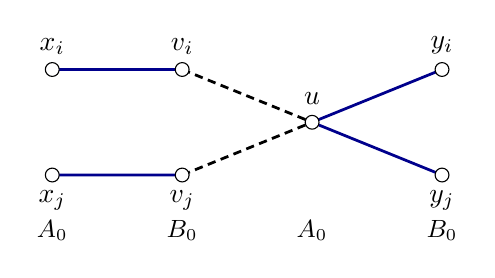
\begin{tikzpicture}[x=1.65cm,y=.67cm,
  vertex/.style={circle,draw,fill=white,inner sep=1.3pt,minimum size=5pt},
  reserve/.style={line width=1pt,blue!55!black},
  matched/.style={line width=1pt,densely dashed}]
  \coordinate (xi) at (0,1); \coordinate (xj) at (0,-1);
  \coordinate (vi) at (1,1); \coordinate (vj) at (1,-1);
  \coordinate (u) at (2,0);
  \coordinate (yi) at (3,1); \coordinate (yj) at (3,-1);
  \draw[reserve] (xi)--(vi) (xj)--(vj) (u)--(yi) (u)--(yj);
  \draw[matched] (vi)--(u) (vj)--(u);
  \foreach \name in {xi,xj,vi,vj,u,yi,yj} \node[vertex] at (\name) {};
  \foreach \name/\lab in {xi/x_i,vi/v_i,yi/y_i}
     \node[above=2pt] at (\name) {$\lab$};
  \foreach \name/\lab in {xj/x_j,vj/v_j,yj/y_j}
     \node[below=2pt] at (\name) {$\lab$};
  \node[above=3pt] at (u) {$u$};
  \foreach \col/\side in {0/$A_0$,1/$B_0$,2/$A_0$,3/$B_0$}
     \node[font=\small] at (\col,-2.05) {\side};
\end{tikzpicture}
\caption{Two colors can pass through the same left vertex \(u\). In color \(i\), the dashed edge \(v_i u\) belongs to the old matching, and the two solid edges are reserve copies. The lower walk makes the corresponding repair in color \(j\), using different reserve copies. Within a color, a second walk through the same matched vertex would reuse its old matching edge.}\label{fig:repair}
\end{figure}

\subsection{A factorization criterion using the nibble}

For the ordinary vertices, suppose the two physical sides each have size \(N\). Let \(C\) be a pool of ordinary crossing copies disjoint from the reserve \(R\). For specified free ordinary sets \(F_i,G_i\), the incidence hypergraph has one vertex for each left demand \((i,x)\) with \(x\in F_i\), one for each right demand \((i,y)\) with \(y\in G_i\), and one for each copy \(e\in C\). Each eligible use of a copy \(e=xy\) gives the triple
\[
 \{(i,x),(i,y),e\}.
\]
Eligibility requires \(x\in F_i\) and \(y\in G_i\). A demand degree counts eligible copies. A copy degree counts eligible colors. A codegree can exceed one only for two opposite demands in the same color, when there are parallel eligible copies between their endpoints.

We use the nibble estimate from Keevash~\cite[Section~3.1]{KeevashII}, in the equal-weight form derived from Ehard, Glock and Joos~\cite{EGJ}. Fix \(0<\delta<1\). For \(\Delta\) sufficiently large in terms of \(\delta\), let the incidence hypergraph have maximum degree at most \(\Delta\), codegrees at most \(\Delta^{1-\delta}\), and all demand degrees at least \((1-\eta)\Delta\), where \(0\le\eta<1\). If the number of triples and the number of tests are each at most \(\exp(\Delta^{(\delta/450)^2})\), there is a matching leaving uncovered mass at most
\[
 B(z)=\max\left\{(\eta+\Delta^{-\delta/450})z,\frac{3\Delta^\delta}{1-\eta}\right\}
 \label{eq:nibble-error}\tag{N}
\]
in every chosen test supported on demands, with weights in \([0,1]\) and total mass \(z\).

\begin{theorem}[Factorization from weighted reserves and a nibble]\label{thm:hybrid-completion}
Fix \(0<\delta<1\). Let \(M\) be a \(D\)-regular multigraph with a balanced cut and equally many ordinary vertices on each side. Its internal edges have a proper coloring with \(k\le D\) colors, leaving equally many free vertices on each side in every color.

Designate separate crossing copies for the exceptional rows in the two orientations, an ordinary pool \(C\), and a simple \(d\)-regular ordinary reserve \(R\), with \(d>0\). At each pair the sum of the designated copies is at most its multiplicity in \(M\). The two orientations of exceptional rows have the following weighted Hall certificates. For a row \(x\), let \(\eta_x\ge0\) be its charge per spent copy. Its weight at an ordinary column is between zero and \(\eta_x\) times the designated multiplicity at that pair. The total weight of a column is at most a common positive bound. In each color a free exceptional row has weight on the free ordinary columns at least that bound plus \((k-1)\eta_x\). The sufficient estimates \eqref{eq:rowx} and \eqref{eq:rowy} give such certificates when measured on the designated copies.

Suppose that after any feasible choice of exception-to-ordinary matchings covering all free exceptions and respecting their designated copies, the following conditions hold on the remaining free ordinary sets \(F_i,G_i\).
\begin{enumerate}
\item For some \(\Delta\) sufficiently large in terms of \(\delta\) and some \(0\le\eta<1\), the incidence hypergraph of \(C\) satisfies the degree and codegree bounds for \eqref{eq:nibble-error}. Both its number of triples and \(2N(k+1)\) are at most \(\exp(\Delta^{(\delta/450)^2})\).
\item The normalized matrix of \(R\) has norm at most \(\sigma<1\) on mean-zero vectors. Every physical vertex has at most \(\beta d\) reserve neighbors outside the opposite free set of any color. For an integer \(h\ge1\) with \(\sigma^h\le1/(2N)\), the quantities
\[
 \ell=2h+1,\qquad t=B(k),\qquad \rho=\beta+B(d)/d
\]
satisfy \eqref{eq:spectral-repair}.
\end{enumerate}
Then the \(k\) internal colors extend to perfect matchings with pairwise disjoint crossing copies, and \(M\) has a 1-factorization.
\end{theorem}

\begin{proof}
The weighted Hall argument from Theorem~\ref{thm:factor} covers the exceptional vertices. In each orientation, the at most \(k-1\) earlier colors can reduce a row's weight by at most \((k-1)\eta_x\). The remaining row and column bounds give Hall's inequality. The two orientations cover disjoint sets of vertices in each color because each joins an exception to an ordinary vertex. They remove the same number of vertices on each side of the cut, leaving \(|F_i|=|G_i|\).

We use two kinds of indicator tests for the nibble. For each physical vertex, we count its demands across the palette, with at most \(k\) demands. For each color and each physical vertex, we count the opposite free demands among its reserve neighbors, with at most \(d\) demands. There are \(2N(k+1)\) tests. The matching of triples gives initial matchings \(M_i\) in \(C\) with distinct physical copies across all the colors. The first tests bound the number of free missed sets containing any vertex by \(B(k)\). The second tests bound the number of newly missed ordinary neighbors by \(B(d)\) at each vertex in each color. Adding the previously unavailable neighbors gives the bound \(\beta d+B(d)=\rho d\) for the missed sets of Lemma~\ref{lem:spectral-repair}.

The lemma completes the ordinary matchings. Their copies and the copies used by the exceptional matchings fit the designated capacities at every physical pair. Together with the internal edges they give \(k\) disjoint perfect matchings. The residue has degree \(D-k\) and contains only crossing copies, so the regular bipartite residue factors by Hall's theorem.
\end{proof}

Hall's theorem supplies the exceptional matchings from the row and column bounds. The ordinary demand degrees and reserve neighborhoods depend on which vertices those matchings use. A bound on the losses that holds for every feasible matching therefore lets us apply the ordinary estimates to the choice supplied by Hall. If each side loses at most \(s\) ordinary vertices, each vertex of a simple pool loses at most \(s\) neighbors on the opposite side. Deleting eligible triples preserves the upper bounds on the copy degrees and codegrees. We use these bounds on the grid below.

\subsection{A sparse grid family outside the rectangle test}\label{sec:sparse-reserve-example}

Fix integers \(b\ge1\) and even \(q\ge12\). Each side has \(N=bq^2\) ordinary vertices on a \(q\)-by-\(q\) grid with \(b\) vertices per cell. We number rows and columns from \(0\) to \(q-1\). Two opposite vertices are adjacent in the grid support when they share a row or a column. Each support pair has one copy in \(C\) and another in \(R\), so both pools have degree \(d=b(2q-1)\). On cell-constant vectors the support matrix is \(b(J_q\otimes I_q+I_q\otimes J_q-I_{q^2})\), where \(J_q\) is the all-ones matrix. The eigenvalue on constants is \(d\). If exactly one coordinate function has sum zero, the eigenvalue is \(b(q-1)\). If both have sum zero, the eigenvalue is \(-b\). On vectors with sum zero in each cell the matrix is zero. Hence the normalized reserve has mean-zero norm \((q-1)/(2q-1)<1/2\).

We put \(d\) copies on one internal pair on the left and on one on the right. The pairs use columns \(0,1\) in row \(0\) on the left and in row \(q/2\) on the right. One copy of each pair goes into each of \(k=d\) colors. The internally free ordinary vertices are paired across the cut by equal coordinates wherever possible. The two remaining left coordinates in row \(q/2\) are paired with the two remaining right coordinates in row \(0\) in their respective columns. Each pair of this bijection receives \(d\) filler copies.

There are \(r=\lfloor\sqrt q\rfloor\) exceptions per side, paired across the cut. For each exceptional pair \(x,y\) we choose two distinct equal-coordinate filler pairs \(u_L,u_R\) in row \(q/2+1\), with the \(2r\) coordinates distinct across the exceptions. This is possible since \(2r\le q\). At either chosen coordinate the \(d\) filler copies are replaced by \(d\) copies each of \(u_Ly\) and \(xu_R\). We also put \(d\) copies on \(xy\). The replacements preserve each ordinary degree, which is \(3d\) from the two grid pools and the internal or filler copies. An exception has two ordinary neighbors of multiplicity \(d\) and its exceptional partner of multiplicity \(d\), so it too has degree \(3d\).

\paragraph{The hybrid parameters.}
Each exceptional row can assign weight \(d\) to its two ordinary neighbors, with column bound \(d\) and charge one. These neighbors are initially free in all colors and each column belongs to a single row in either orientation. After any feasible matching of the exceptions, each free ordinary side has size \(N-r-2\). A physical vertex loses at most \(r+2\) neighbors in either grid pool. Thus the incidence hypergraph has maximum degree at most \(d\), codegree at most one, and demand degrees at least \(d-r-2\). The number of triples is at most \(kNd\), and the number of tests is \(2N(k+1)\), both polynomial in \(q\).

We take \(\Delta=k=d\), \(\delta=1/4\), and \(\eta=\beta=(r+2)/d\). With \(b\) fixed, \(\eta=O(d^{-1/2})\), and
\[
 \frac{B(d)}{d}
 =\max\left\{\eta+d^{-1/1800},\,\frac{3d^{-3/4}}{1-\eta}\right\}
 =O(d^{-1/1800}).
\]
Thus \(t/d\) and \(\rho\) are both \(O(d^{-1/1800})\). Taking \(h=\lceil\log_2(2N)\rceil\) gives \(\ell=O(\log N)\). Since \(k=d\), the two left sides of \eqref{eq:spectral-repair} are bounded by \(O((\log N)^2d^{-1/1800})=o(1)\). This calculation gives the asymptotic application of Theorem~\ref{thm:hybrid-completion}.

\begin{corollary}[Grid factorization and rectangle separation]\label{cor:sparse-grid}
For every \(b\ge1\) and even \(q\ge12\), the multigraph just constructed has a 1-factorization. It has \(d=\Theta(\sqrt N)\) distinct ordinary crossing neighbors at each ordinary vertex and \(r=\Theta(N^{1/4})\) exceptions per side for fixed \(b\). The rectangle criterion of Theorem~\ref{thm:factor} fails for every admissible internal palette on this cut.
\end{corollary}

\begin{proof}
The explicit threshold comes from the filler pairs. In each of the \(d\) rounds we use one copy of each internal edge. At the first switched coordinate for \(x,y\), we match \(u_L\) to \(y\) and \(x\) to \(u_R\), using fresh copies in each round. The second switched coordinate for each pair of exceptions is still uncovered on both sides. Call it a hole. A hole can exchange its missing filler with any grid neighbor whose diagonal filler is intact. Excluding the four internal endpoint coordinates and all \(2r\) switched coordinates leaves at least \(d-(2r+4)\) choices at every hole.

We show that the exchanges can be scheduled whenever
\[
 r\le m_0=\left\lceil\frac d2\right\rceil
 \qquad\text{and}\qquad
 \left\lfloor\frac d2\right\rfloor\ge 2r+4.
\]
Each hole then has at least \(m_0\) eligible helpers. For each hole we select exactly \(m_0\) of them. This gives a simple bipartite graph of degree \(m_0\) at every hole and degree at most \(r\le m_0\) at every helper. By K\H{o}nig's bipartite edge-coloring theorem, these pairs split into \(m_0\) matchings. Every matching covers every hole, and the helpers used in a round are distinct. For \(q\ge12\), we have \(q\ge2r+5\). For \(r\le3\) this follows from \(q\ge12\), and for \(r\ge4\) it follows from \(q\ge r^2\). Since \(\lfloor d/2\rfloor\ge q-1\), both inequalities hold for every \(b\ge1\).

We duplicate the schedule, assigning the two occurrences to the two different grid pools, and keep \(d\) of the \(2m_0\) rounds. If a hole at coordinate \(z\) uses a helper at \(w\), its exchange uses \(z_Lw_R\) and \(w_Lz_R\). Both grid pairs exist because sharing a row or column is symmetric. The exchanges in a round are disjoint, and the pool and endpoint coordinates of a copy identify its hole, helper, and direction. Each hole uses a given helper at most once in each pool, so every copy used by an exchange is distinct. The unused helpers and the two off-diagonal filler pairs use separate copies of their fillers in each round. This gives \(d\) disjoint perfect matchings containing the internal copies. The residue is \(2d\)-regular and bipartite, so it factors.

For separation, let \(S\) be the left first half of the rows and \(T\) the right second half. They have total size \(N\). In either direction, a vertex of this rectangle sees \(bq/2\) vertices in the other half through its column and uses two grid copies at each. The filler copies on equal coordinates and the two fillers directed from the second half on the left to the first half on the right contribute zero to the rectangle. Thus every vertex has \(bq<d\) copies to the opposite set. A proper internal coloring needs at least \(d\) colors because each internal pair has \(d\) parallel copies. The rectangle exceeds the threshold \(N-r-2a\) of Theorem~\ref{thm:factor}, and its copies per vertex are fewer than the size of every admissible palette. The ordinary crossing support is exactly the grid support, since the off-diagonal fillers share a column. For fixed \(b\), the expressions for \(N,d,r\) give the stated growth rates.
\end{proof}

The grid separates the rectangle test from factorability on the specified cut. The explicit threshold \(q\ge12\) uses the filler matching to schedule deterministic exchanges. Theorem~\ref{thm:hybrid-completion} uses the bulk and reserve pools under the degree and spectral hypotheses, which hold for this grid for all sufficiently large \(q\) at fixed \(b\).
